\documentclass{article}


\usepackage{arxiv}

\usepackage[utf8]{inputenc} % allow utf-8 input
\usepackage[T1]{fontenc}    % use 8-bit T1 fonts
\usepackage{hyperref}       % hyperlinks
\usepackage{url}            % simple URL typesetting
\usepackage{booktabs}       % professional-quality tables
\usepackage{amsfonts}       % blackboard math symbols
\usepackage{nicefrac}       % compact symbols for 1/2, etc.
\usepackage{microtype}      % microtypography
\usepackage{lipsum}
\usepackage{graphicx}

\title{Pseudo-Boolean Encoding for Local Envy Freeness}


\author{
  Jean-Guy Mailly\\
  LIPADE -- Université de Paris\\
  Paris, France\\
  \texttt{jean-guy.mailly@u-paris.fr} \\
  %% examples of more authors
   \And
Nicolas Maudet \\
LIP6 -- Sorbonne University\\
Paris, France\\
\texttt{nicolas.maudet@lip6.fr} \\
\And
Anaelle Wilczynski\\
  Affiliation \\
  Address \\
  \texttt{anaelle.wilczynski@centralesupelec.fr} \\
  %% \And
  %% Coauthor \\
  %% Affiliation \\
  %% Address \\
  %% \texttt{email} \\
  %% \And
  %% Coauthor \\
  %% Affiliation \\
  %% Address \\
  %% \texttt{email} \\
}

\begin{document}
\maketitle

\begin{abstract}
\lipsum[1]
\end{abstract}


\section{Introduction}
See \cite{BeynierCGHLMW19}.

\section{Problem Formulation}
\begin{itemize}
	\item $O = \{o_1, \dots, o_n\}$: set of objects
	\item $N = \{1,\dots,n\}$: set of agents
	\item $\succ_i$: preferences of agent $i$ over $O$ (linear order)
	\item $G = \langle N, E\rangle$: social network (undirected graph)
\end{itemize}
{\bf Problem:} assign each agent $i$ an object $o_k$ s.t. $i$ does not prefer the object assigned to one of her neighbors, {\em i.e.} $\forall j \in N$ s.t. $\{i,j\} \in E$, $i$ does not prefers $o_l$ to $o_k$, where $o_l$ is the object assigned to $j$.

\section{Pseudo-Boolean Encoding for the Decision Problem}
\subsection{First Step: SAT Encoding}
Boolean variables:
\begin{itemize}
	\item $\forall i \in N, o_k, o_l \in O$, $pref_i^{o_k,o_l} = \top$ iff $o_k \succ_i o_l$,
	\item $\forall i \in N, o \in O$, $alloc_{i,o} = \top$ iff $o$ is allocated to $i$.
\end{itemize}

Model the allocation:
\[
\phi_{alloc} = \bigwedge_{i \in N} (\bigoplus_{o \in O} alloc_{i,o}) \wedge \bigwedge_{o \in O} (\bigoplus_{i \in N} alloc_{i,o})
\]

Model Local Envy-freeness:
\[
\phi_{lef} = \bigwedge_{\{i,j\} \in E} (\bigwedge_{o_k,o_l \in O} (alloc_{i,o_k} \wedge alloc_{j,o_l}) \rightarrow pref_i^{o_k,o_l}) \equiv \bigwedge_{\{i,j\} \in E} (\bigwedge_{o_k,o_l \in O} \neg alloc_{i,o_k} \vee \neg alloc_{j,o_l} \vee pref_i^{o_k,o_l})
\]

\subsection{Second Step: PB Encoding}
XOR are easy to encode as Pseudo-Boolean constraints. $\phi_{alloc}$ is replaced by the set of PB constraints:
\begin{description}
	\item[($PB_{alloc}^{i}$)] $\sum_{o \in O} alloc_{i,o} = 1$
	\item[($PB_{alloc}^{o}$)] $\sum_{i \in N} alloc_{i,o} = 1$
\end{description}

Clauses can be easily encoded as PB constraints as well. So $\phi_{lef}$ is replaced by the set of PB constraints:
\begin{description}
	\item[$(PB_{lef}^{i,j,o_k,o_l})$] $\neg alloc_{i,o_k} + \neg alloc_{j,o_l} + pref_i^{o_k,o_l} \geq 1$
\end{description}
where $\{i,j\} \in E$.

\section{Preliminary Experimental Evaluation for DEC-LEF}\label{section:expe-dec-lef}
\subsection{Implementation and Experimental Environment}
\begin{itemize}
	\item Sat4j \cite{BerreP10} used for solving the PB instance
	\item Python script used for reading the allocation instance (social network $+$ preferences), providing the PB encoding, and parsing the output of Sat4j
	\item Experimental environment: macOS 11.5, M1 SoC (3.2GHz), 8Go RAM
\end{itemize}

\subsection{Random Social Network}
\subsubsection{Protocol}
\begin{itemize}
	\item Social networks: Erdos-Renyi graphs with probability $p \in \{0.3, 0.5, 0.7\}$
	\item For each $p$ and each size $n \in \{10,20,30,40,50\}$, $10$ instances are generated
	\item The preferences of each agent are a random shuffle of the list of objects $[o_1,\dots,o_n]$
\end{itemize}

\subsubsection{Results}
\begin{figure}[htb]
\centering
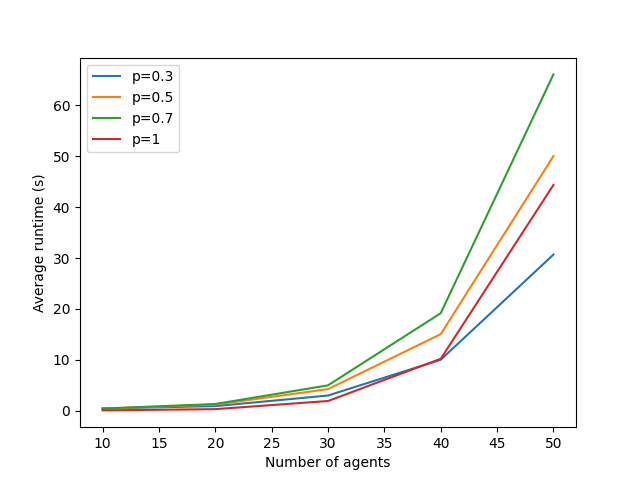
\includegraphics[width=0.5\linewidth]{results.png}
\caption{Preliminary Results for DEC-LEF: Average Runtime on Random Graphs for $n \in \{10,20,30,40,50\}$}
\end{figure}

\subsection{Line Social Network}
\begin{itemize}
	\item Line made of $n \in \{10, 20, 30, 40, 50\}$ agents
	\item The preferences of each agent are a random shuffle of the list of objects $[o_1,\dots,o_n]$
\end{itemize}

\subsubsection{Results}
\begin{figure}[htb]
\centering
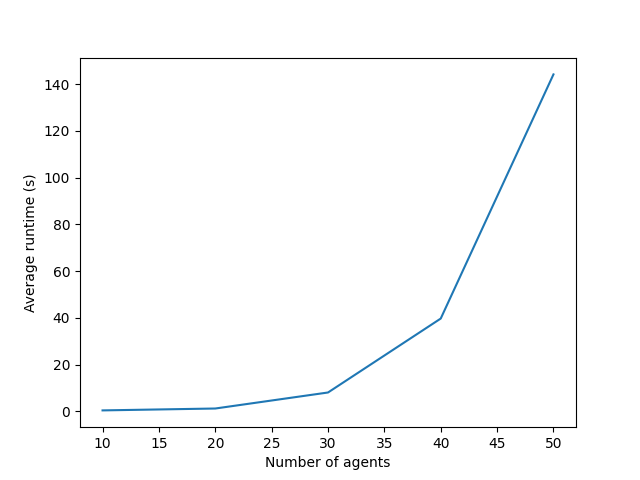
\includegraphics[width=0.5\linewidth]{results_line.png}
\caption{Preliminary Results for DEC-LEF: Average Runtime on Lines for $n \in \{10,20,30,40,50\}$}
\end{figure}

\section{Pseudo-Boolean Encoding for the Optimization Problem}
\begin{itemize}
	\item $O = \{o_1, \dots, o_n\}$: set of objects
	\item $N = \{1,\dots,n\}$: set of agents
	\item $\succ_i$: preferences of agent $i$ over $O$ (linear order)
	\item $G = \langle N, E\rangle$: social network (undirected graph)
\end{itemize}
{\bf Problem:} assign each agent $i$ an object $o_k$ s.t. the number of LEF agents is maximal.
%$i$ does not prefer the object assigned to one of her neighbors, {\em i.e.} $\forall j \in N$ s.t. $\{i,j\} \in E$, $i$ does not prefers $o_l$ to $o_k$, where $o_l$ is the object assigned to $j$.

The encoding is almost the same as in the previous case, except that the constraint
\begin{description}
	\item[$(PB_{lef}^{i,j,o_k,o_l})$] $\neg alloc_{i,o_k} + \neg alloc_{j,o_l} + pref_i^{o_k,o_l} \geq 1$
\end{description}
%where $\{i,j\} \in E$.
is replaced by
\begin{description}
	\item[$(PB_{lef}^{i,j,o_k,o_l})$] $\neg alloc_{i,o_k} + \neg alloc_{j,o_l} + pref_i^{o_k,o_l} + non\_lef_i \geq 1$
\end{description}
where $non\_lef_i$ is a newly introduced Boolean variable which is true iff the agent $i$ is not LEF: the variable is assigned $\top$ in order to satisfy the constraint in the case where the rest of the constraint is not satisfy. Then, an objective function is added:
\begin{description}
	\item[(Obj)] \verb+minimize+ $\sum_{i \in N} non\_lef_i$
\end{description}

\section{Preliminary Experimental Evaluation for MAX-LEF}
\subsection{Implementation and Protocol}
Same as Section~\ref{section:expe-dec-lef}.

\subsection{Results}
\begin{figure}[htb]
\centering
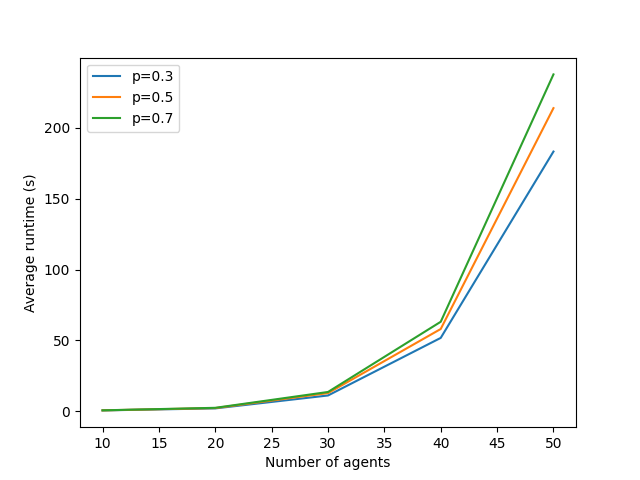
\includegraphics[width=0.5\linewidth]{results_optim.png}
\caption{Preliminary Results for MAX-LEF: Average Runtime for $n \in \{10,20,30,40,50\}$}
\end{figure}

\section{Ideas}
Easy ones:
\begin{itemize}
	\item Preferential attachment for generating the graphs
	\item Study the ratio of yes/no instances
	\item Study the cost of the optimal solutions
	\item Can we complete a partial allocation into a LEF allocation?
	\item Can we obtain a LEF allocation with a given set of forbidden pairs agent/object?
\end{itemize}

Harder ones:
\begin{itemize}
	\item Constraint on the preferences (single peaked,...)
	\item MUS of the UNSAT instances (explicability of negative results)
	\item $k$-local envy freeness (look at the $k$ neighbors)
	\item Use the non-envy graph
	\item Sequence of swaps (from a given allocation, can we reach a LEF allocation?)
	\item Variant: each agent can have several objects, each object has an utility, and she is envy-free if the sum of the utilities is greater or equal to the sum of the utility of her neighbors' bundle
	\[
	\sum_{o_k} alloc_{i,o_k} \times u_{i,o_k} \geq \sum_{o_k} alloc_{j,o_k} \times u_{i,o_k}
	\]
\end{itemize}

\bibliographystyle{unsrt}  
\bibliography{references} 
\end{document}
